% !TEX root = ../main.tex
\documentclass[../main.tex]{subfiles}


\begin{document}

\section{Computer Boot Process}
\label{sec:computer-boot-process}

\subsection{Overview}
Upon powering up a computer, it undergoes a predetermined sequence of steps known as the \texttt{boot process}.
The boot process responsibilities encompass:
\begin{itemize}
  \item Locating and initializing hardware devices
  \item Loading and executing the operating system bootloader
  \item Providing configuration wizard for configuring onboarding devices
\end{itemize}

First step is to initialize the CPU and memory. Then CPU executes
code at a fixed memory location, known as the \texttt{reset vector}.
For \texttt{x86} architecture, the reset vector is at address \texttt{0xFFFFFFF0h} \cite{resetvector}.
At this address, a hardware flash memory known as \texttt{BIOS} is located (figure \ref{fig:uefi_chip}). \texttt{BIOS} is a firmware
that initializes the hardware and loads the bootloader. The bootloader is a small program that
loads the operating system kernel into memory and executes it. The operating system kernel
is the base component of operating system which manages the hardware and provides functions for
accessing the hardware.

On modern computers, the \texttt{BIOS} is replaced by \texttt{UEFI} (Unified Extensible Firmware Interface) \cite{uefi_spec}.
UEFI is a specification that defined a software interface between the operating system and the platform firmware.
It is designed to replace the \texttt{BIOS} firmware interface. \texttt{UEFI} is a more capable firmware which supports:
\begin{itemize}
  \item Secure boot
  \item Network boot \footnote{Network boot is a process of providing boot configuration and code over network}\footnote{It is also possible to network boot computer that uses BIOS}
  \item Booting from large disks \footnote{Larger than 2.2 TB \cite{bios_limits}}
  \item Booting from disks with GUID Partition Table (GPT)
  \item Booting from disks with more than 4 physical partitions
\end{itemize}

\begin{figure}[H]
  \centering
  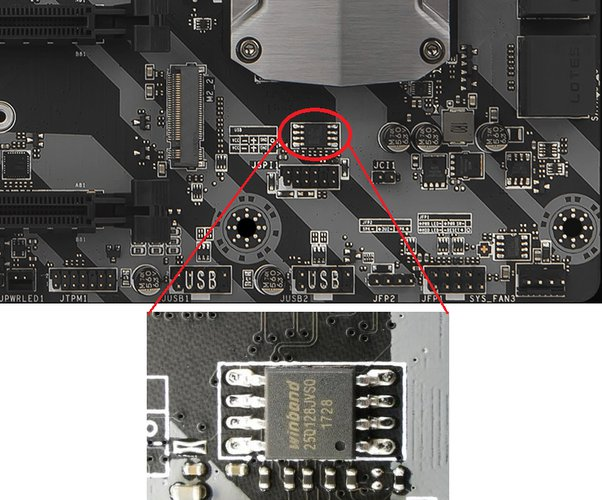
\includegraphics[width=\textwidth]{uefi_chip.jpg}
  \caption{Flash memory on motherboard containing UEFI firmware \cite{uefi_chip_img_ref}}
  \label{fig:uefi_chip}
\end{figure}

\subsection{Network booting}
\label{subsec:network-booting}

Network booting involves initiating the boot process of a computer through a network rather than its local disk.
This method of booting is often supported by \texttt{UEFI}/\texttt{BIOS} firmware via the
\texttt{PXE} (Preboot Execution Environment) protocol \cite{pxespec}. The \texttt{PXE} protocol
describes the client-server (figure \ref{fig:pxe_client_server_model}) interactions that take place during the boot process.
For the client to participate in the network boot process, it needs to have a \texttt{PXE} capable network interface controller (NIC).

On the server side, a \texttt{DHCP} (Dynamic Host Configuration Protocol) server with \texttt{PXE} extensions is required
alongside a \texttt{TFTP} (Trivial File Transfer Protocol) server. The \texttt{DHCP} server provides the client with
information about the location of the \texttt{TFTP} server and the URI of the boot image to load from the \texttt{TFTP} server.

\begin{figure}[H]
  \centering
  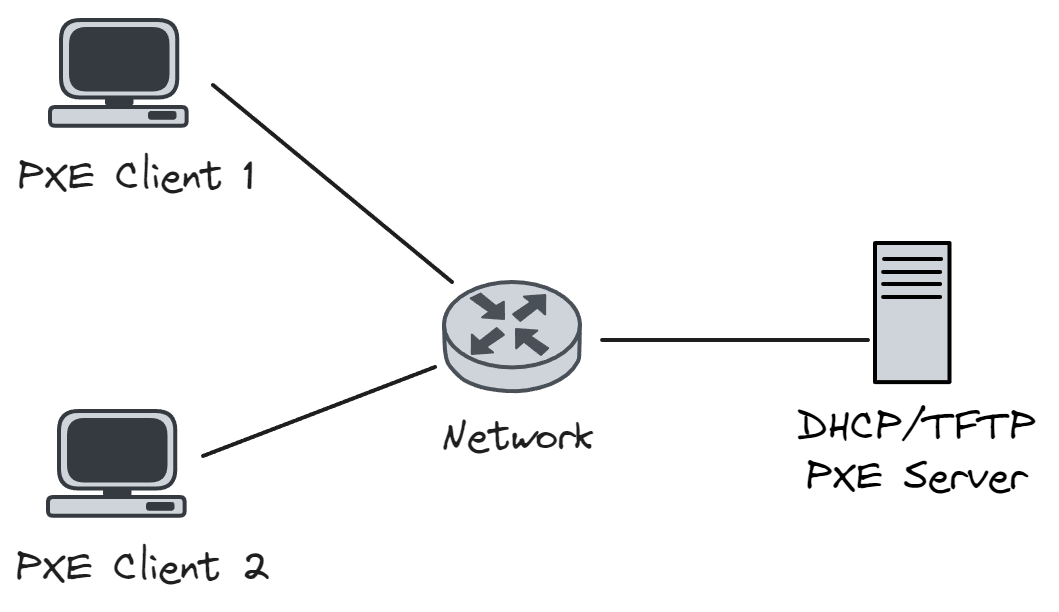
\includegraphics[width=\textwidth]{pxe/client_server_model.png}
  \caption{Client-server model of PXE protocol \cite{pxespec}}
  \label{fig:pxe_client_server_model}
\end{figure}

\begin{figure}[H]
  \centering
  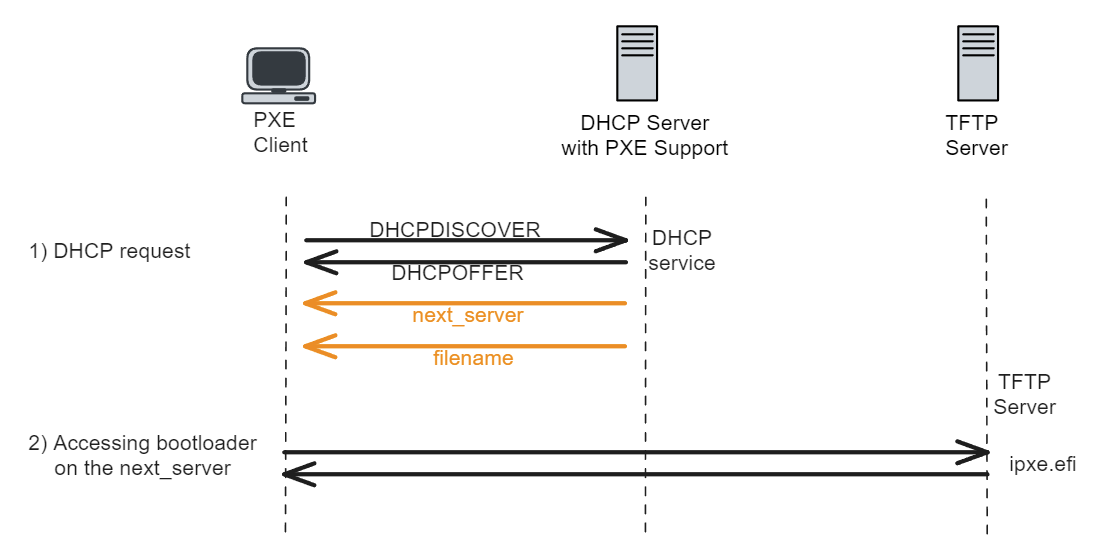
\includegraphics[width=\textwidth]{pxe/protocol.png}
  \caption{PXE client-server communication protocol \cite{pxespec_protocol}}
  \label{fig:pxe_protocol}
\end{figure}

The PXE client-server communication shown in figure \ref{fig:pxe_protocol} starts with the client
broadcasting a \texttt{DHCP} request. The \texttt{DHCP} server responds with a \texttt{DHCP} offer
containing additional \texttt{PXE} information as shown in figure \ref{fig:pxe_dhcp_offer}.

% TODO: Would be useful to crop top 3 pixels of this image to remove the black line
%       this can be achieved using tools like nbconvert
\begin{figure}[H]
  \centering
  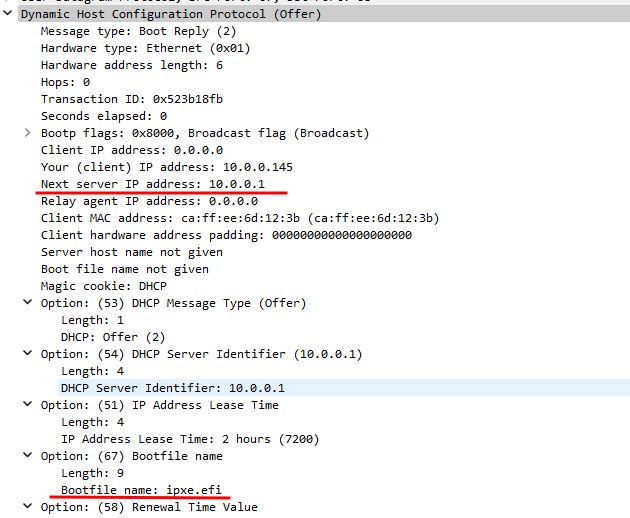
\includegraphics[width=\textwidth]{pxe/dhcp-pxe-capture.png}
  \caption{DHCP offer packet with PXE extensions \cite{pxespec_dhcp_options}}
  \label{fig:pxe_dhcp_offer}
\end{figure}

Selected \texttt{DHCP} options from figure \ref{fig:pxe_dhcp_offer}:

\begin{itemize}
  \item \texttt{Next Server IP address} - This refers to the IP address of the \texttt{TFTP} server, commonly denoted as \texttt{next\_server} in \texttt{DHCP} configuration files
  \item \texttt{Boot File Name} - This refers to the URI of the boot image to load from the \texttt{TFTP} server, commonly denoted as \texttt{filename} in \texttt{DHCP} configuration files
\end{itemize}

Using the information from the \texttt{DHCP} offer, the client then sends a \texttt{TFTP} file retrieval command to the \texttt{TFTP} server.
The \texttt{filename} option from the \texttt{DHCP} offer is used as the file path in the TFTP request.
After successfully retrieving the boot image, the client executes the boot image. Which will handle the rest of the boot process.
This usually involves loading the operating system kernel alongside the initial ramdisk into memory and executing the kernel.

\section{Project Objective}

The objective of this project is to create software designed for the remote management and configuration of computers.
It will be built upon the described network booting process and seek to offer a practical solution for the issues outlined in section \ref{sec:motivation-and-background}.

\end{document}